\section{Data and Parameters}
\label{sec:data_and_parameters}

The model is described by a large number of parameters that govern the number of
contacts a person has, the likelihood of becoming infected on each contact, the
likelihood of developing light or strong symptoms or even dying from the disease as well
as the duration each stage of the disease takes.

Most of these parameters can be calibrated from existing datasets or the medical
literature or calibrated from surveys and empirical datasets.

\subsection{Medical Parameters}

This section discusses the medical parameters used in the model, their sources and how we arrived at the distributions used in the model.\footnotemark

\footnotetext{Additional information can be found in the \href{https://sid-dev.readthedocs.io/en/latest/reference_guides/epi_params.html}{online documentation}.}


\subsubsection{Length of Presymptomatic Stage / Incubation Period}


Estimates of the incubation period usually give a range from 2 to 12 days. A meta analysis by \citet{McAloon2020} comes to the conclusion that ``The incubation period distribution may be modeled with a lognormal distribution with pooled $\mu$ and $\sigma$ parameters (95\% CIs) of 1.63 (95\% CI 1.51 to 1.75) and 0.50 (95\% CI 0.46 to 0.55), respectively.'' For simplicity we discretize this distribution into four bins.


\subsubsection{Begin of Infectiousness}

The period between infection and onset of infectiousness is called latent or latency period. However, the latency period is rarely given in epidemiological reports on Covid-19. Instead, scientists and agencies usually report the incubation period, the period from infection to the onset of symptoms. A few studies used measurements of virus shedding to estimate infectiousness during the course of the disease. When measurements started before the onset of symptoms the development of the viral load before symptoms gives us an indication of number of days between the onset of infectiousness and symptoms.

The European Centre for Disease Prevention and Control estimates that people become infectious between one and two days before the symptoms set in. This is similar to \citet{He2020} who estimate this to take 2.3 days and is in line with \citet{Peak2020}.

Given these numbers and the length of the incubation period we can calculate the latency period for symptomatic people. To our knowledge no estimates for the latency period of asymptomatic cases of COVID-19 exist. We assume it to be the same for symptomatic and asymptomatic cases.

Thus, we arrive at the following distribution for latency periods: 40\% have one day. 35\% have two days. 20\% have three days and 5\% have 5 days.


\subsubsection{Duration of Infectiousness}

We assume that the duration of infectiousness is the same for both symptomatic and asymptomatic individuals as evidence suggests little differences in the transmission rates of SARS-CoV-2 virus between symptomatic and asymptomatic patients (\citet{Yin2020}) and that the viral load between symptomatic and asymptomatic individuals are similar (\citet{Zou2020}, \citet{Byrne2020}, \citet{Singanayagam2020}).

Our distribution of the duration of infectiousness is based on \citet{Byrne2020}.

For symptomatic cases they arrive at 0-5 days before symptom onset (figure 2) and 3-8 days of infectiousness afterwards.\footnote{Viral loads may be detected much later but 8 days seems to be the time after which most people are culture negative, as also reported by \citet{Singanayagam2020}} Thus, we arrive at 0 to 13 days as the range for infectiousness among individuals who become symptomatic (see also figure 5). This duration range is very much in line with the meta-analysis’ reported evidence for asymptomatic individuals (see their figure 1). Thus, we arrive at 0 to 13 days as the range for infectiousness among individuals who become symptomatic. This duration range is very much in line with the meta-analysis' reported evidence for asymptomatic individuals.

Following this evidence we assume the following discretized distribution of the infectiousness period: 10\% of individuals are infectious for three days, 25\% for five days, another 25\% for seven days, 20\% for nine days and 20\% for eleven days.


\subsubsection{Duration of Symptoms}

We use the duration to recovery of mild and moderate cases reported by \cite[Figure~S3, Panel~2]{Bi2020} for the duration of symptoms for asymptomatic and non-ICU requiring symptomatic cases.

We collapse the data to the following distribution: 10\% recover after 15 days and 30\% require 18, 22 or 27 days respectively.

These numbers are only used for mild cases. We do not disaggregate by age. Note that the length of symptoms is not very important in our model given that individuals stop being infectious before their symptoms cease.


\subsubsection{Time from Symptom Onset to Admission to ICU}

The data on how many percent of symptomatic patients will require ICU is pretty thin. We rely on data by the US CDC (\citet{Stokes2020}) and \href{https://github.com/BDI-pathogens/OpenABM-Covid19/blob/572e24ca2dbf7153789a92ad3a27e4c515d0e576/documentation/parameters/parameter_dictionary.md}{the OpenABM-Project}. Table~\ref{tab:symptomatic-to-ICU} shows our derivations for the probabilities of requiring intensive care per age group.

\begin{table}[tb]
    \caption{Shares of symptomatic patients who will require ICU care by age groups.}
    \label{tab:symptomatic-to-ICU}
    \centering

    \begin{tabular}{ll}
        \toprule
        Age Group & Share \\
        \midrule
        0-9 & 0.00005 \\
        10-19 & 0.00030 \\
        20-29 & 0.00075 \\
        30-39 & 0.00345 \\
        40-49 & 0.01380 \\
        50-59 & 0.03404 \\
        60-69 & 0.10138 \\
        70-79 & 0.16891 \\
        80-100 & 0.26871 \\
        \bottomrule
    \end{tabular}

    \tablenotes{The data is taken from \citet{Stokes2020} and \href{https://github.com/BDI-pathogens/OpenABM-Covid19/blob/572e24ca2dbf7153789a92ad3a27e4c515d0e576/documentation/parameters/parameter_dictionary.md}{the OpenABM-Project}.}

\end{table}

For those who will require intensive care we follow \citet{Chen2020} who estimate the time from symptom onset to ICU admission as 8.5 $\pm$ 4 days.

This aligns well with numbers reported for the time from first symptoms to hospitalization: \citet{Gaythorpe2020} report a mean of 5.76 with a standard deviation of 4. This is also in line with the durations collected by \href{https://www.rki.de/DE/Content/InfAZ/N/Neuartiges_Coronavirus/Steckbrief.html#doc13776792bodyText16}{the Robert Koch Institut}.

We assume that the time between symptom onset and ICU takes 4, 6, 8 or 10 days with equal probabilities. These times mostly matter for the ICU capacities.


\subsubsection{Death and Recovery from ICU}

We take the survival probabilities and time to death and time until recovery from intensive care from the \href{https://tinyurl.com/y5owhyts}{OpenABM Project}.

They report time until death to have a mean of 11.74 days and a standard deviation of 8.79 days. Approximating this with the normal distribution, we have nearly 10\% probability mass below 0. We use it nevertheless as several other distributions (such as chi squared and uniform) were unable to match the variance.
Discretizing this leads to 41\% of individuals who die from Covid-19 to die after one day in intensive care. 22\% day after 12 days, 29\% after 20 days and 7\% after 32 days. Again, we rescale this for every age group among those that will not survive.

They report time until recovery to have a mean of 18.8 days and a standard deviation of 12.21 days. Approximating this with the normal distribution, we have over 5\% probability mass below 0. Discretizing this of those who recover in intensive care 22\% do so after one day, 30\% after 15 days, 28\% after 25 days and 18\% after 45 days.

\FloatBarrier

\subsection{The Synthetic Population}

We build a synthetic population based on the German microcensus \citep{FDSAeDBUDL2018}.
We only use private households, i.e. exclude living arrangements such as nursing homes as
non-private households vary widely in size and it is very difficult to know which
contacts take place in such living arrangements.

We sample households to build our synthetic population of over one million households
keeping for each individual their age, gender, occupation and whether they work on
Saturdays and Sundays. For each household we draw its county and set the corresponding
federal state.% we draw the county because county is not part of the campus file

We randomly assign 35\% of children below three to attend a nursery \citep{Destatis2020}.
For children between three and six years old, we assume all go to preschool (officially
92.5\% according to \cite{Destatis2020}). Nursery groups consist

Children that attend a nursery meet in groups of four plus one adult care taker every
weekday when there are no school vacations. Preschool children meet in groups of nine
with two adult care takers. These groups are mixed with respect to age but all belong to
the same state and mostly to the same county. For nurseries the group size is four, for
preschools it's nine \citep{BertelsmannStiftung2019}.

Every child that goes to school is part of three different classes that meet every day on
weekdays when there are no vacations and no school policies are in place.\footnote{We
implement vacations on the federal state level.} Each class consists of approximately 23
students \citep{OECD2013} and two teachers. All students in a class are of the same age
and live in the same state and if mostly also in the same county. In addition, each
child gets assigned a value that captures his or her need to attend nursery, preschool or
school. This allows us to capture various degrees of emergency care that can be granted
while educational facilities are closed or function in some kind of rotating schedule.

Workers are assigned to a daily meeting work group. The group sizes vary to match the
number of daily repeating work contacts reported by working individuals in
\cite{Mossong2008}. These groups only consist of workers that work in the same county.
For a distribution of the number of daily recurring work contacts see
Figure~\ref{n_contacts_work_daily_recurrent}. To match the number of weekly work groups
we match each worker with up to 14 other workers to match the number of reported weekly
work contacts shown in Figure~\ref{n_contacts_work_weekly_recurrent}. Each pair is
assigned a weekend on which they always meet in the absence of work policies. 80\% of
these contacts are individuals from the same county.
% work contact priority
In the same way children have a educational priority determining if they are entitled to
emergency care workers are assigned a work contact priority that captures how necessary
their work is and to which degree they can work from home. This means that it's always
the same individuals that continue to have work contacts when work from home mandates of
a certain strictness are in place. Since our work contact priority is uniformly normal
from zero to one, we can use the reduction in work mobility as reported by
\cite{Google2021} as a proxy for the share of individuals that do not have work contacts.

In addition to creating groups for educational facilities and work we also have other
recurring contacts to represent things like groups of friends or sports teams that
practice regularly together. Both daily and weekly groups are created analogously to the
work groups but matching the numbers in Figure~\ref{n_contacts_other_daily_recurrent} and
Figure~\ref{n_contacts_other_weekly_recurrent}. In addition, since leisure contacts are
highly assortative by age all individuals that have a daily leisure contact are matched
with a person not only from the same county but also from the same age group.

The individuals in our population can react to events such as developing symptoms that
are typical of CoViD-19, a positive PCR test or a positive rapid test by reducing their
contacts. To determine who would reduce their contacts in such a situation or demand a
rapid test to avoid quarantine we introduce a quarantine compliance parameter. Similarly
we introduce a rapid test compliance parameter that determines in which order individuals
start demanding rapid tests when rapid tests become increasingly available. This makes
sure that when for example only 10\% of workers get tested, it's the same workers that
have access to tests every week.

Lastly, for the distribution of vaccinations every individual is assigned a vaccination
group and a vaccination rank from that group that creates a complete vaccination queue
over the population including 15\% that refuse to be vaccinated \citep{RKI2021}. The
vaccination groups are created to match the recommendations by the Ständige
Impfkommission \citep{VygenBonnet2020}.\footnote{We cover that teachers were prioritized
more than recommended by the commission.}\comment[id=K]{Write how that plays out in our simulations for the different age groups.}

% To cover that the Pfizer-BioNTech vaccine was later approved for younger age groups we
% put adolescents and children into two groups that follow after the general population.
% These groups do not become eligible within our simulation frame until June.


% \begin{figure}[ht]   % vaccinations by age group
%   \centering
%   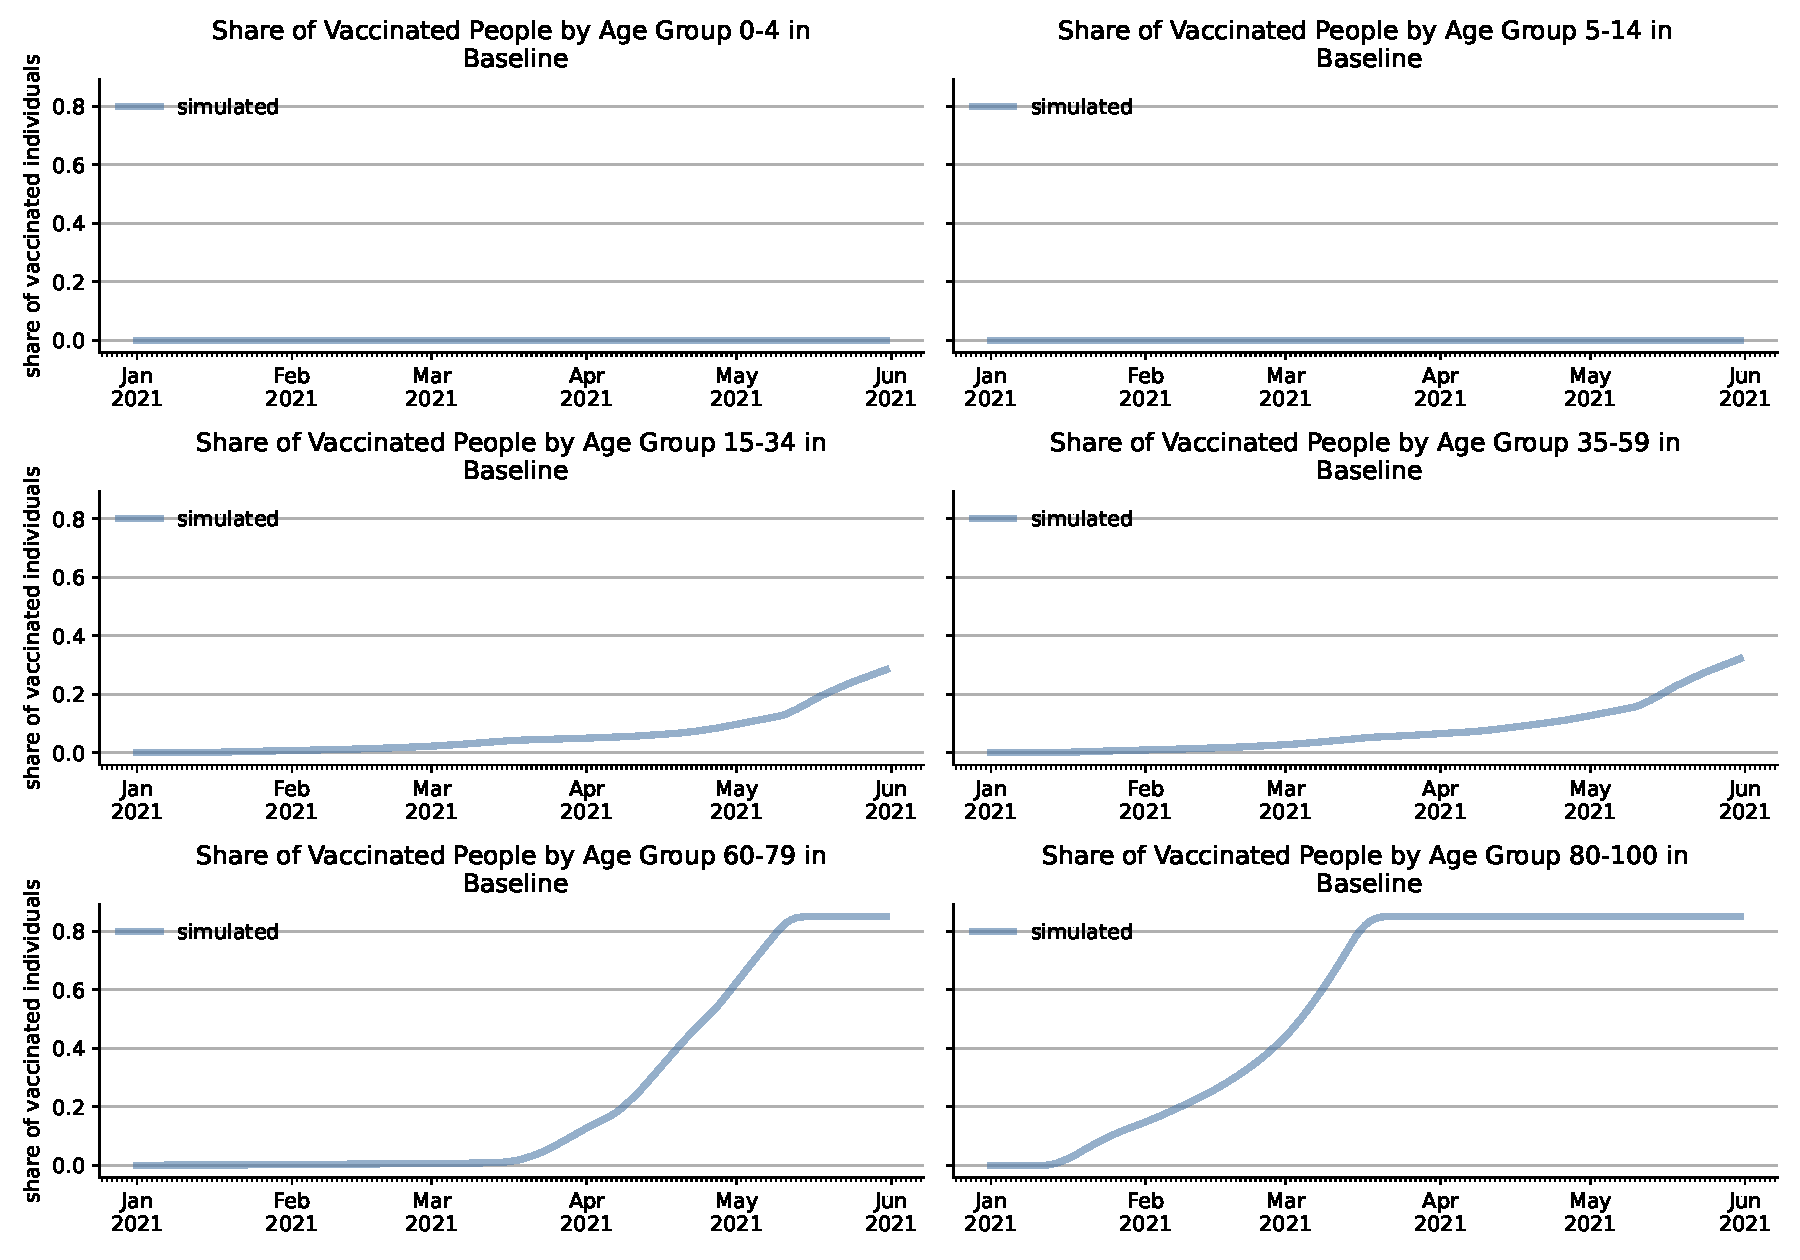
\includegraphics[width=\textwidth]{figures/results/figures/vaccinations/spring_baseline}
%   \caption{Simulated and Empirical Infections by Federal State}
%   \floatfoot{\noindent \textit{Note:} \textcolor{red}{To be written.}}
%   \label{fig:vaccinations_by_age_group}
% \end{figure}


\FloatBarrier


\subsection{Number of Contacts}
\label{subsec:data_number_of_contacts}

We calibrate the parameters for the predicted numbers of contacts from contact diaries
of over 2000 individuals from Germany, Belgium, the Netherlands and Luxembourg
\citep{Mossong2008}. Each contact diary contains all contacts an individual had
throughout one day, including information on the other person (such as age and gender)
and information on the contact. Importantly, for each contact individuals entered of
which type the contact (school, leisure, work etc.) was and how frequent the contact
with the other person is.

Simplifying the number of contacts, we arrive at the following distributions of the
numbers of contacts by contact type.

\begin{figure}
    \centering

    \begin{subfigure}[b]{0.25\textwidth}
        \centering

        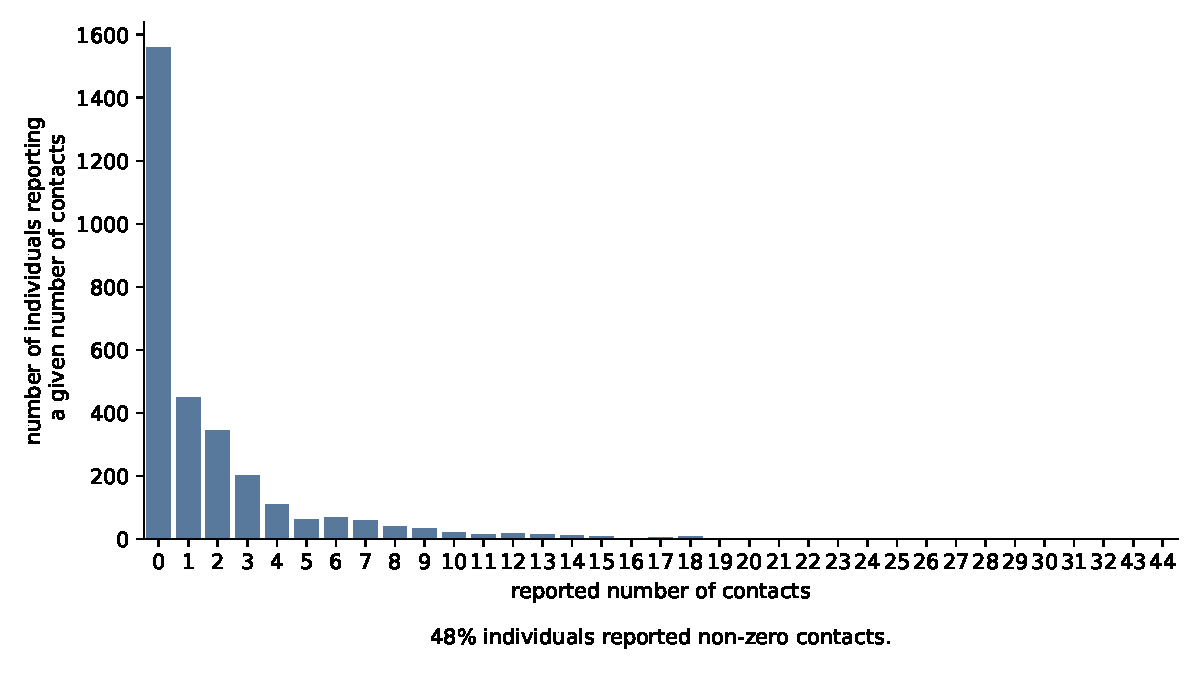
\includegraphics[width=\textwidth]{figures/results/figures/data/distributions_of_the_number_of_contacts/other_non_recurrent}
        \caption{Number of Non Recurrent Other Contacts}
        \label{n_contacts_other_non_recurrent}
    \end{subfigure}

    \hfill

    \begin{subfigure}[b]{0.25\textwidth}
        \centering
        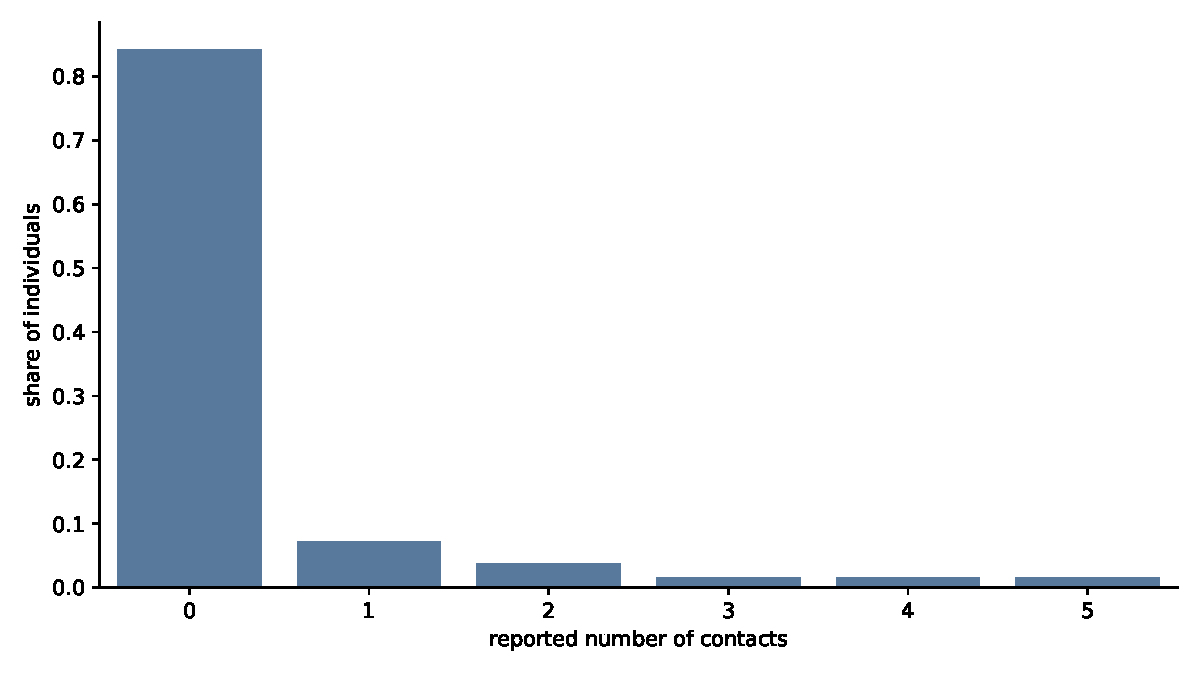
\includegraphics[width=\textwidth]{figures/results/figures/data/distributions_of_the_number_of_contacts/other_recurrent_daily}
        \caption{Number of Daily Recurrent Other Contacts}
        \label{n_contacts_other_daily_recurrent}
    \end{subfigure}

    \hfill

    \begin{subfigure}[b]{0.25\textwidth}
        \centering
        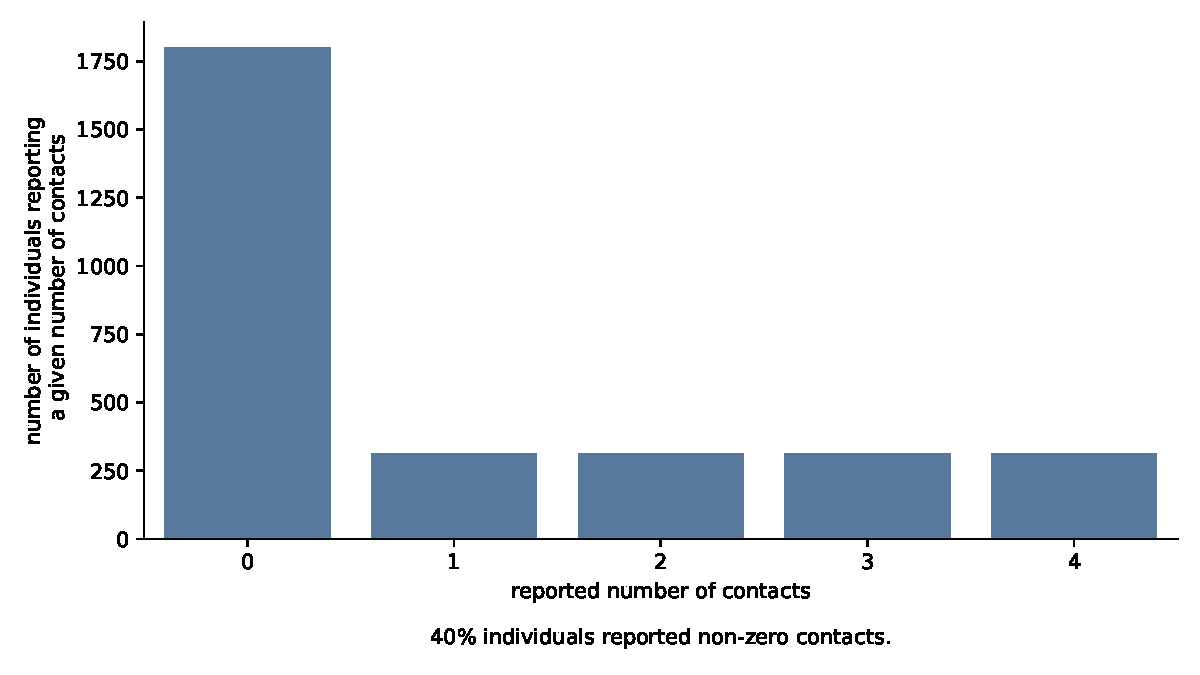
\includegraphics[width=\textwidth]{figures/results/figures/data/distributions_of_the_number_of_contacts/other_recurrent_weekly}
        \caption{Number of Weekly Recurrent Other Contacts}
        \label{n_contacts_other_weekly_recurrent}
    \end{subfigure}

    \vskip3ex
    \caption{Number of Contacts of the Other Contact Type}
    \label{fig:n_contacts_other}

    \floatfoot{\noindent
        \textit{Note:} Other contacts include all contacts that are not household
        members, school contacts or work contacts, for example leisure contacts or
        contacts during grocery shopping. The planned number of contacts is reduced by
        policies, seasonality and individual responses to events such as receiving a
        positive rapid test to the number of actual contacts with transmission potential.        % non recurrent
        In the model it is sampled every day which of the numbers of non recurrent
        contacts a person is planned to have. Note that the contact diaries include such
        high values that super spreading events are well possible in our model through
        non recurrent other models. We assume that individuals in households with
        children or teachers or retired individuals have additional non recurrent
        contacts during school vacations to cover things like family visits or travel
        during vacations. We estimate this to be on average 0.5 additional contacts per
        vacation day.
        % daily and weekly
        For the recurrent other contacts, individuals are assigned to groups that are
        time constant and that meet daily or weekly. The share of individuals who attend
        in a way that has transmission potential is reduced by policies, seasonality and
        individual responses to events such as receiving a positive rapid test. For
        weekly contacts, individuals are assigned to up to four groups that are time
        constant and that meet weekly. The day on which meetings take place varies
        between groups but stays the same for each group.
    }
\end{figure}


% work contacts

\begin{figure}
    \centering
    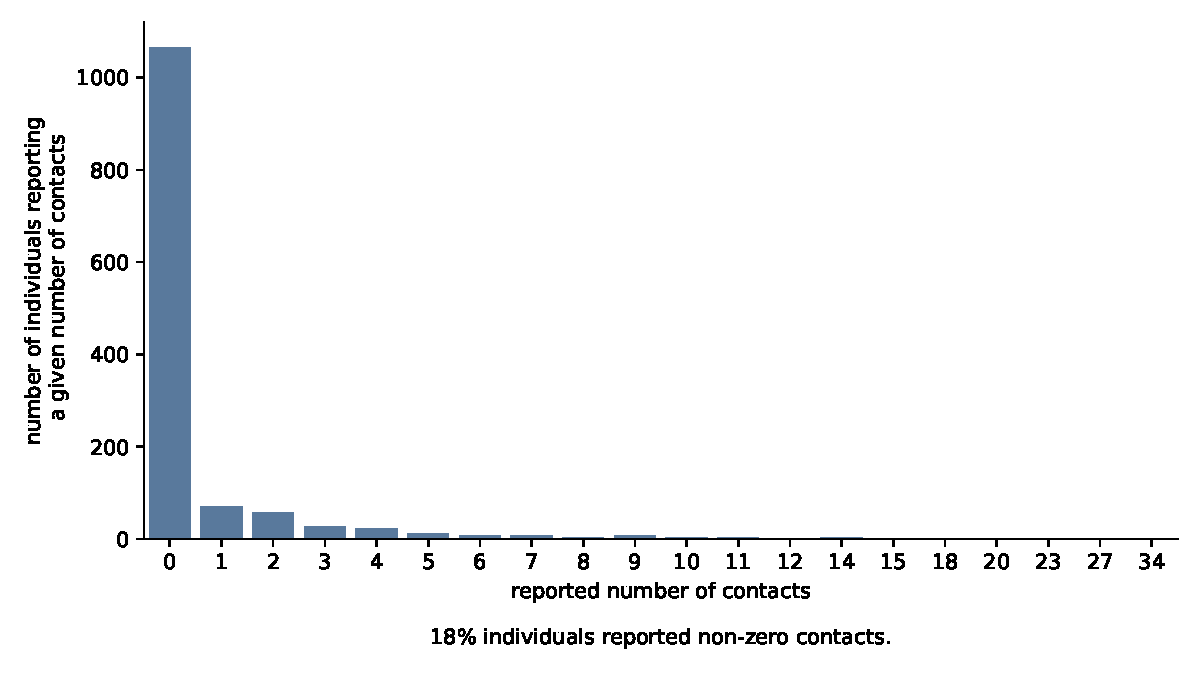
\includegraphics[width=\textwidth]{figures/results/figures/data/distributions_of_the_number_of_contacts/work_non_recurrent}
    \caption{Number of Non Recurrent Work Contacts}
    \label{n_contacts_work_non_recurrent}
    \floatfoot{\noindent \textit{Note:} In the model it is sampled every day which of
        these numbers of contacts a working person is planned to have. Note that the
        contact diaries include such high values that super spreading events are well
        possible in our model. The planned number of contacts is reduced by policies,
        seasonality and individual responses to events such as receiving a positive rapid
        test to the number of actual contacts with transmission potential. Work contacts
        only take place between working individuals.}
\end{figure}


\begin{figure}
    \centering
    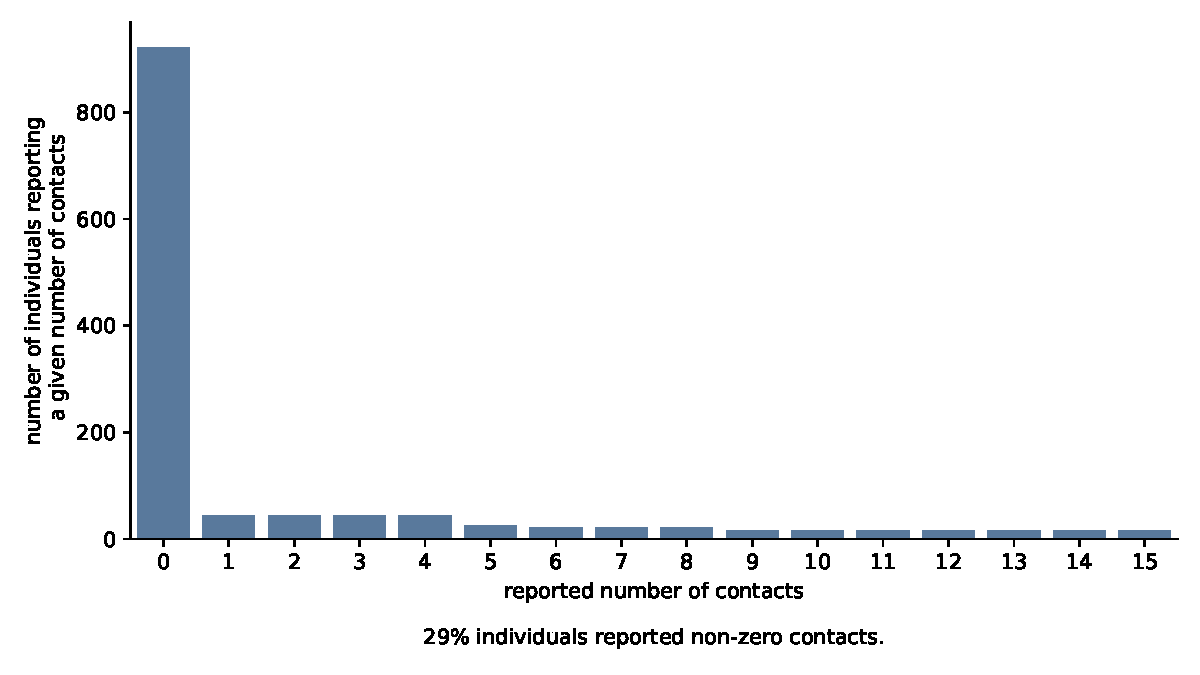
\includegraphics[width=\textwidth]{figures/results/figures/data/distributions_of_the_number_of_contacts/work_recurrent_daily}
    \caption{Number of Daily Recurrent Work Contacts}
    \label{n_contacts_work_daily_recurrent}
    \floatfoot{\noindent \textit{Note:} Working individuals are assigned to groups that
        are time constant and that meet daily to match the given distribution of daily
        work contacts. You can think of these as for example colleagues with which one
        shares an office space. The share of individuals who attend in a way that has
        transmission potential is reduced by policies (such as a work from home mandate),
        seasonality and individual responses to events such as receiving a positive rapid
        test. Work contacts only take place between working individuals.}
\end{figure}


\begin{figure}
    \centering
    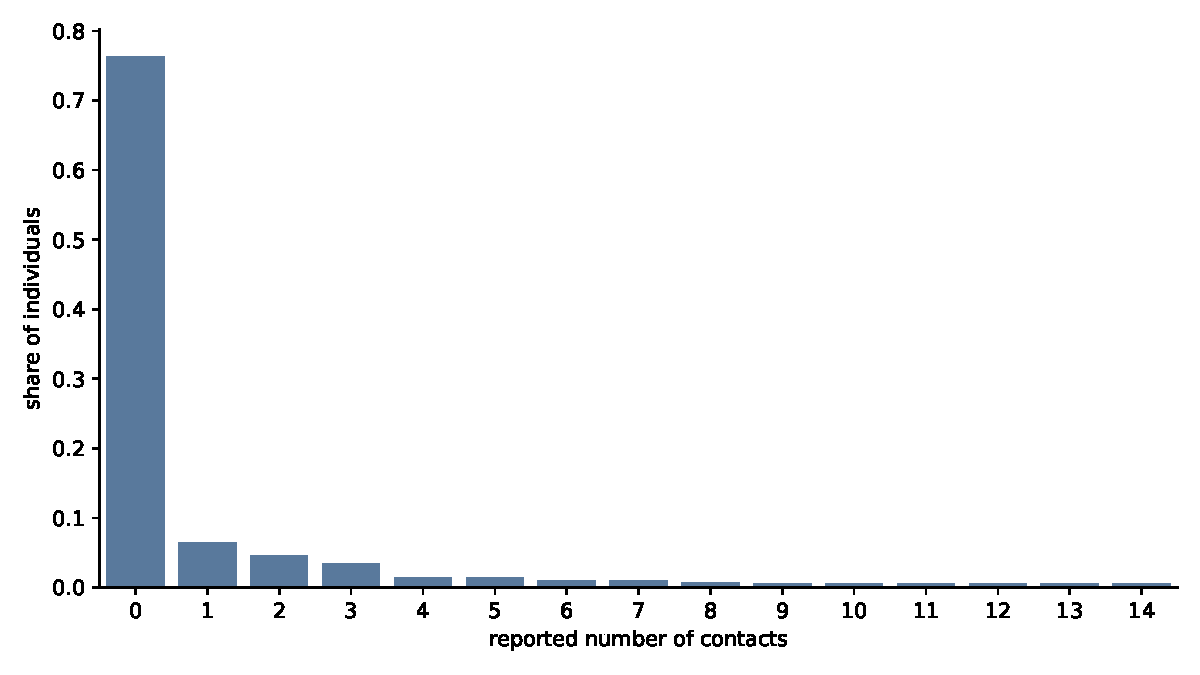
\includegraphics[width=\textwidth]{figures/results/figures/data/distributions_of_the_number_of_contacts/work_recurrent_weekly}
    \caption{Number of Weekly Recurrent Work Contacts}
    \label{n_contacts_work_weekly_recurrent}
    \floatfoot{\noindent  \textit{Note:} Working individuals are assigned to up to 14
        groups that are time constant and meet weekly. Groups are scheduled to meet on
        separate days of the work week. These contact models cover weekly team meetings
        etc. The share of individuals that attend in a way that has transmission
        potential is reduced by policies, seasonality and individual responses to events
        such as receiving a positive rapid test. Work contacts only take place between
        working individuals.}
\end{figure}

An exception where we do not rely on the data by \cite{Mossong2008} are the household
contacts. Since household are included in the the German microcensus
\citep{FDSAeDBUDL2018} on which we build our synthetic population we simply assume for
the household contact model that individuals meet all other household members every day.


\begin{figure}
    \centering
    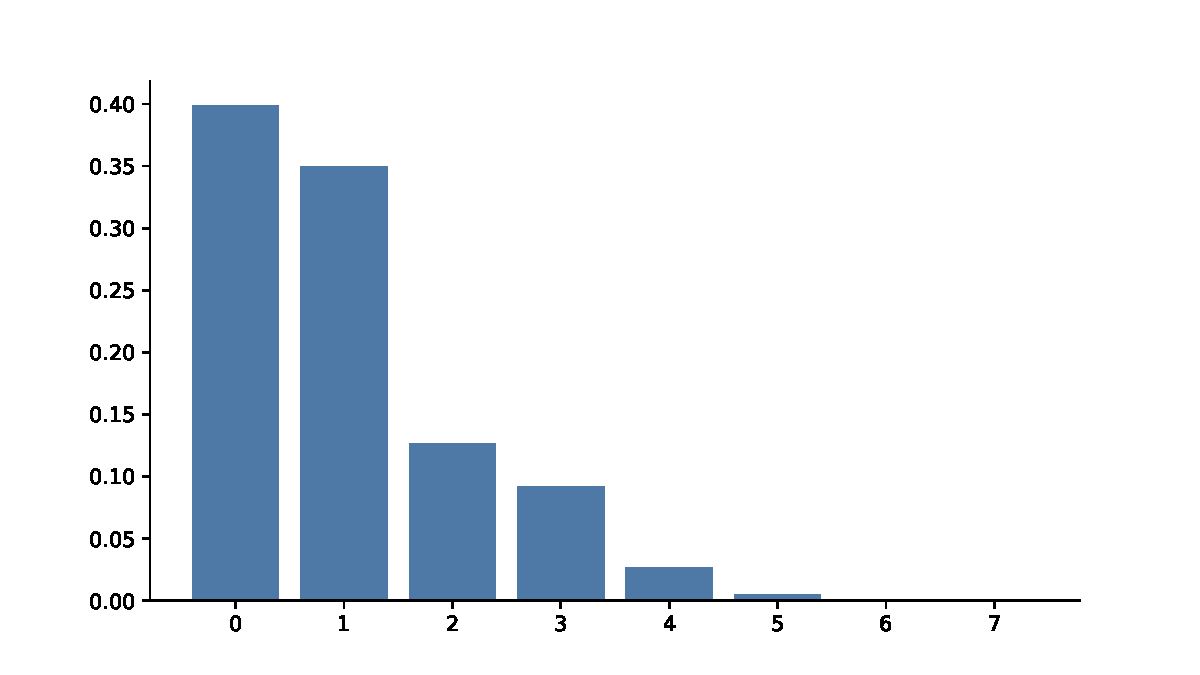
\includegraphics[width=\textwidth]{figures/results/figures/data/distributions_of_the_number_of_contacts/household}
    \caption{Number of Household Contacts}
    \label{n_contacts_hh}
    \floatfoot{\noindent
        \textit{Note:} Every individual meets all other household members every day. The
        German microcensus sampled full households such that our synthetic population
        automatically fits population characteristics such as size and age distribution.}
\end{figure}




\FloatBarrier


\subsection{Contacts by age}
\label{subsec:contacts_by_age}

As mentioned in section \ref{sec:matching}, the probability that two individuals are
matched can depend on background characteristics. In particular, we allow this
probability to depend on age and county of residence. While we do not have good data on
geographical assortativity and just roughly calibrate it such that 80\% of contacts are
within the same county, we can calibrate the assortative mixing by age from the same data
we use to calibrate the number of contacts.

\begin{figure}[ht]
    \centering
    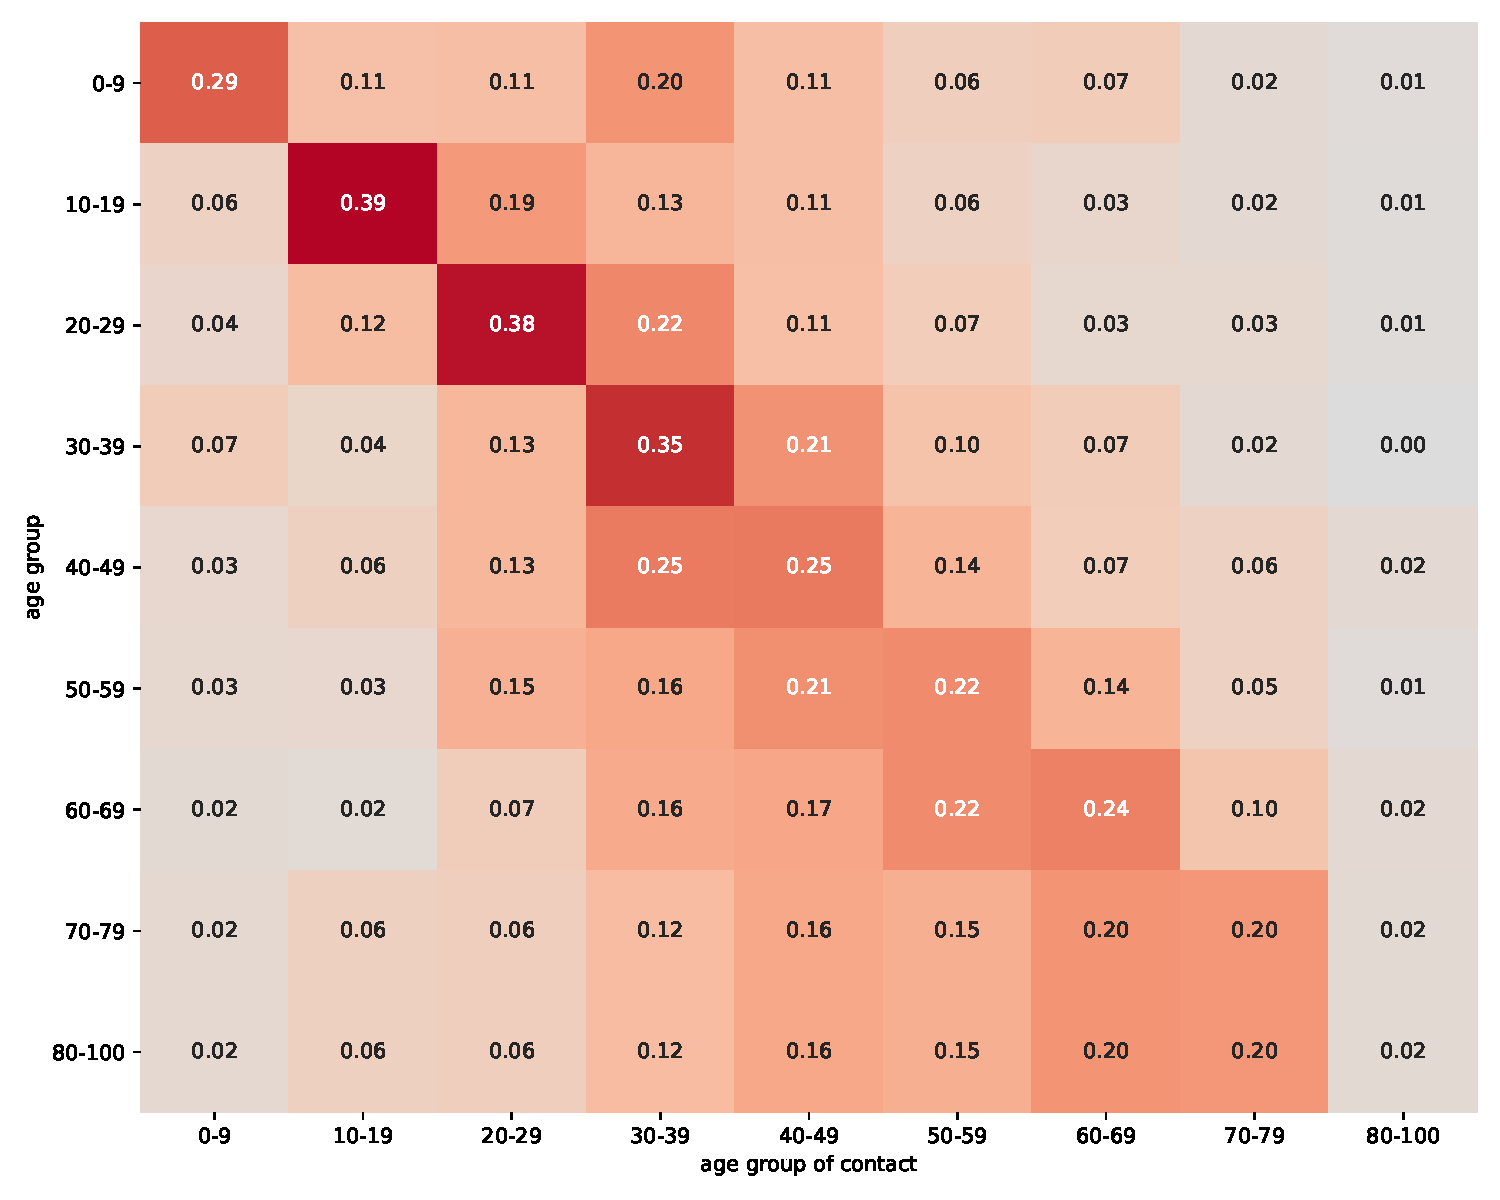
\includegraphics[width=0.9 \textwidth]{figures/results/figures/data/assortativity_other_non_recurrent}
    \caption{Distribution of Non Recurrent Other Contacts by Age Group}
    \label{fig:assortativity_other}
    \floatfoot{\noindent \textit{Note:} The figure shows the distribution of non
        recurrent other contacts by age group. A row shows the share of contacts a
        certain age group has with all other age groups. Higher values are colored in
        darker red tones. The diagonal represents the share of contacts with individuals
        from the same age group.}
\end{figure}


Figure~\ref{fig:assortativity_other} shows that assortativity by age is especially strong
for children and younger adults. For older people, the pattern becomes more dispersed
around their own age group, but within-age-group contacts are still the most common
contacts.

\begin{figure}[ht]
    \centering
    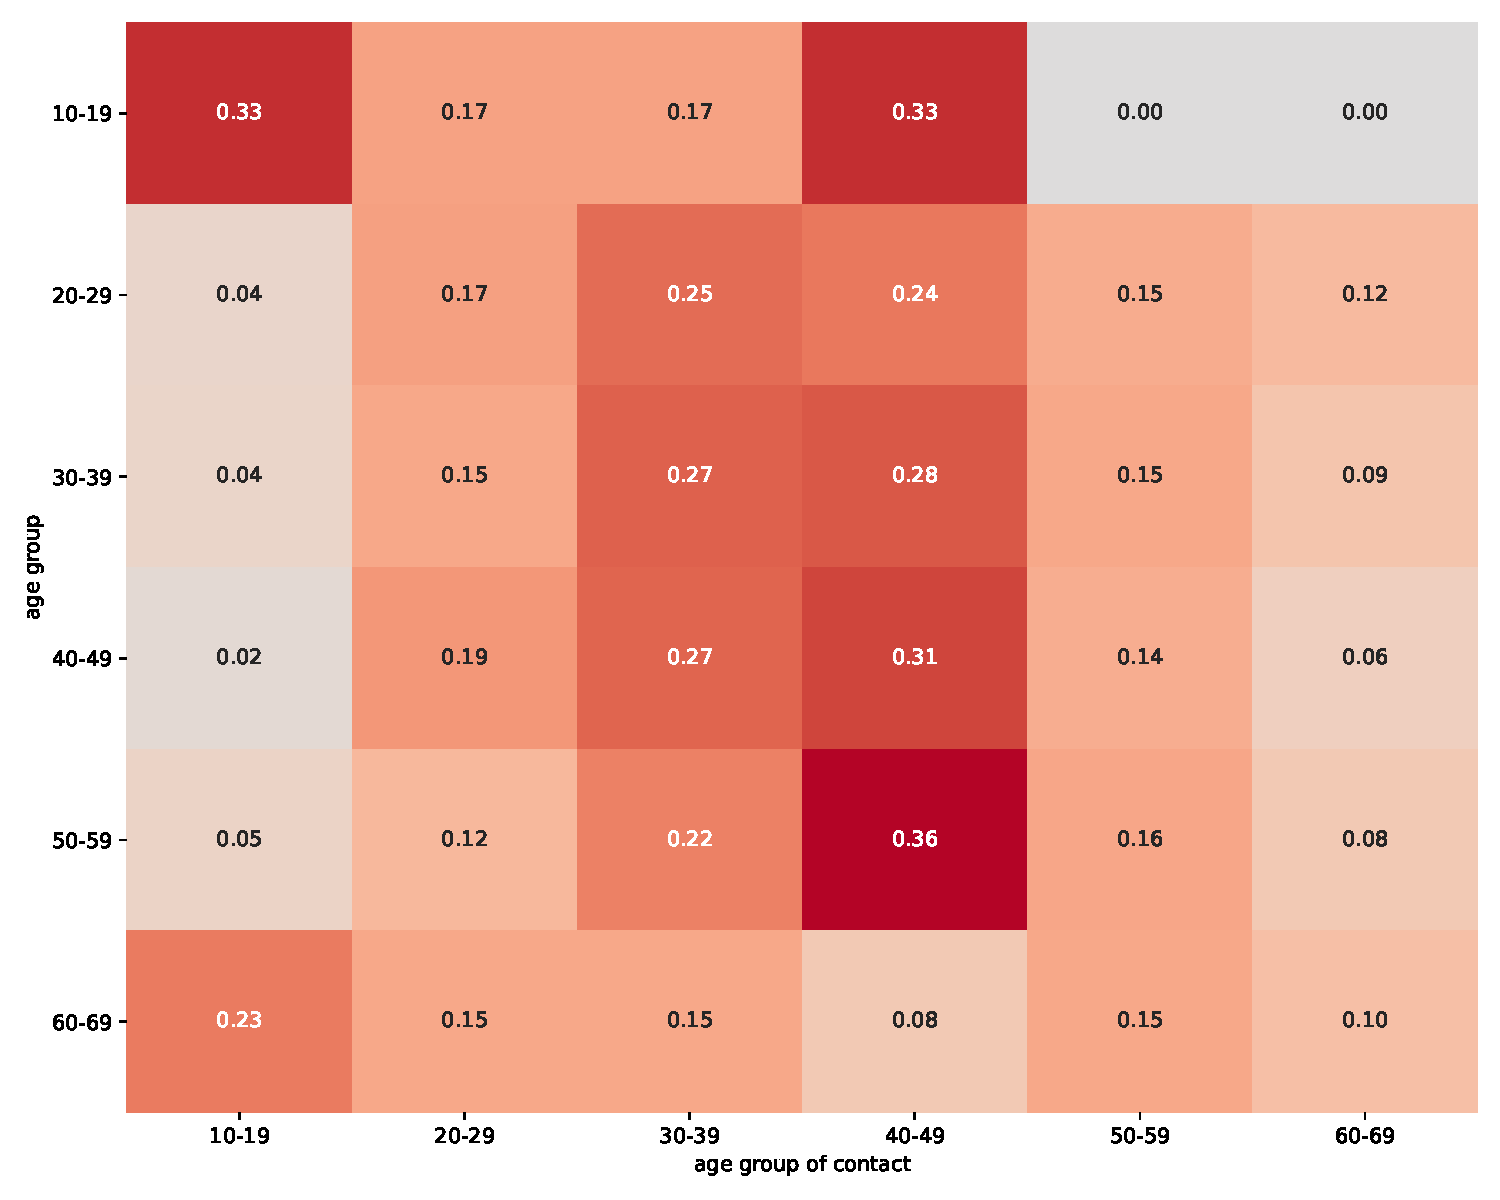
\includegraphics[width=0.9 \textwidth]{figures/results/figures/data/assortativity_work_non_recurrent}
    \caption{Distribution of Random Work Contacts by Age Group}
    \label{fig:assortativity_work}
    \floatfoot{\noindent \textit{Note:} The figure shows the distribution of non
        recurrent work contacts by age group. A row shows the share of contacts a certain
        age group has with all other age groups. Higher values are colored in darker red
        tones. The diagonal represents the share of contacts with individuals from the
        same age group. We only show age groups that have a significant fraction of
        working individuals.}
\end{figure}

Figure~\ref{fig:assortativity_work} shows that assortativity by age is also important
among work contacts.

Our two other types of contacts, households and schools, get their assortativity by
construction. Schools are groups where the same children of the mostly same age and
county meet with teachers every day. Household composition follows directly from the
German microcensus data we use to construct our synthetic population.

\FloatBarrier

\subsection{Policies and Seasonality}
\label{subsec:policies_seasonality}


In our empirical application\comment[id=K]{Improve language} we distinguish four groups
of contact types: households, education, work and other contacts.% households
For households we assume that the individuals'
contacts in their households do not change over our estimation period.
% educ models
For nurseries, preschools and schools we implement vacations as announced by the German
federal states as well as school closures, emergency care and A / B schooling where only
one half of students attends every other week or day. For the moment we ignore that lack
of childcare leads working parents to stay home. An approximation of the share of contacts still taking place with the different school regulations can be found in Figure~\ref{fig:school_multiplier}.

\begin{figure}
    \centering
    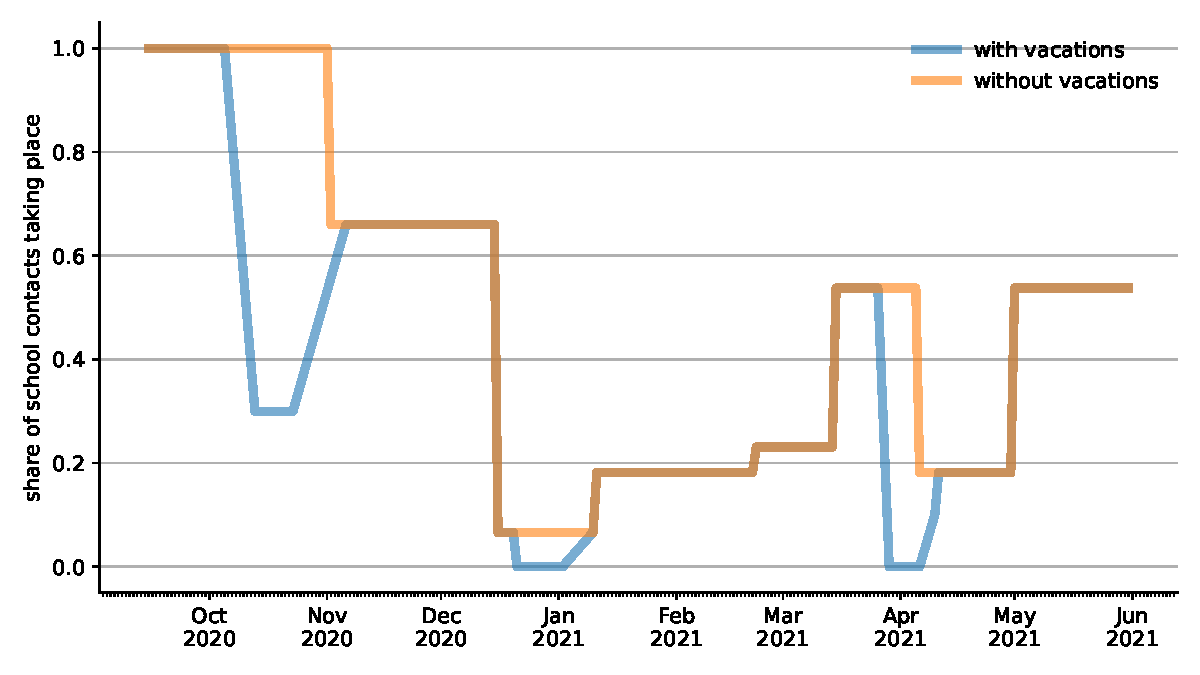
\includegraphics[width=\textwidth]{figures/results/figures/data/school_multiplier_comparison}
    \caption{School Multiplier With and Without Vacations Factored In}
    \floatfoot{\noindent \textit{Note:} The dates on which schools have vacation are
    decided at the federal level. Vacations are directly implemented in our model with no
    school contacts taking place on weekends and during vacations (by federal state) just
    like the schooling mode (full operation, emergency care, rotating schemes with half
    class sizes etc.). The figure is thus only an illustration that roughly shows the
    share of contacts taking place compared to pre-pandemic level with and without
    vacations. The difference between the lines show when vacations take place and to
    what degree. For example all states have fall vacations but the timing varies
    strongly between states.}
    \label{fig:school_multiplier}
\end{figure}


%
% Schließung von Kindertagesstätten und Schulen: 37,4 Millionen ausgefallene Arbeitstage
% http://www.iab-forum.de/schul-und-kitaschliessungen-krankheit-quarantaene-die-coronabedingten-arbeitsausfaelle-der-erwerbstaetigen-steigen-auf-592-millionen-arbeitstage/
%
%
% https://www.sueddeutsche.de/politik/schulschliessung-lockdown-bildung-1.5190377: In
% allen Ländern geht trotz des Lockdowns ein erheblicher Anteil der Schülerinnen und
% Schüler in die Schule.
% https://gfx.sueddeutsche.de/apps/e525337/www/_image_desktopw1840q70-1e2e2bf78b7d4430
% 18% der Grundschüler in Notbetreuung in BW
%

% work
For our work contacts we use the reductions in work mobility reported in the Google
Mobility Data \citep{Google2021} to calibrate our work policies. Reductions in work
contacts are not random but governed through a work contact priority where the policy
changes the threshold below which workers stay home. Figure \ref{fig:work_multiplier}
shows the share of workers that go to work in our model over time.

\begin{figure}[ht]
    \centering
    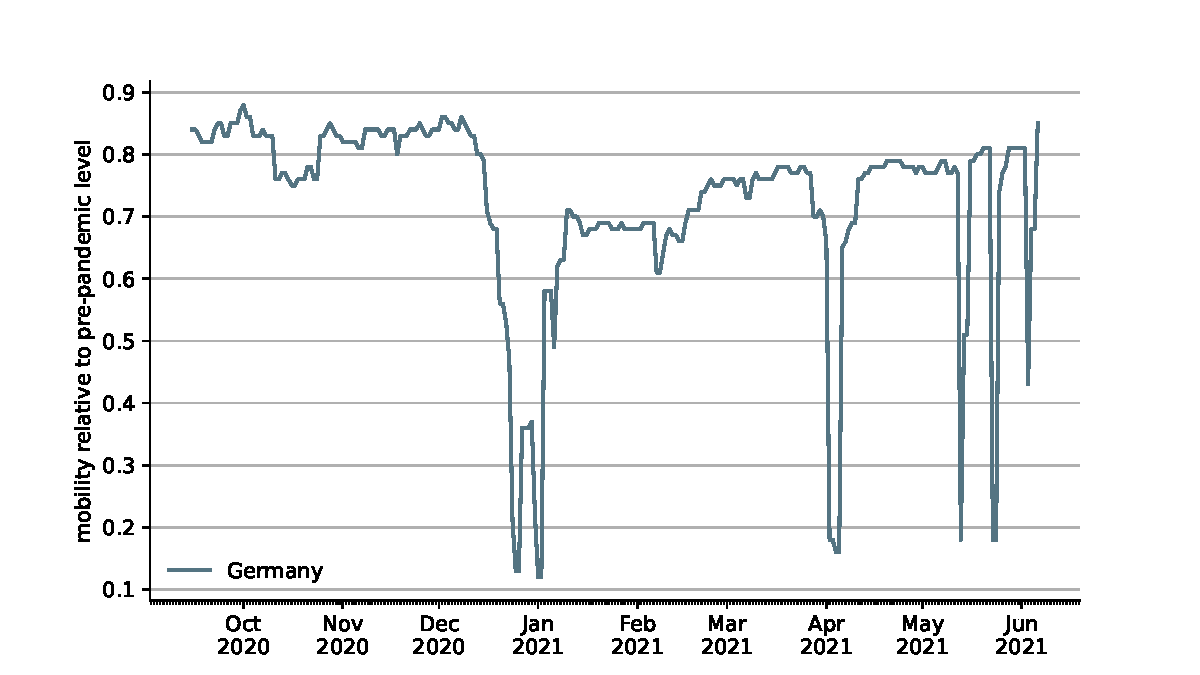
\includegraphics[width=\textwidth]{figures/results/figures/data/work_multiplier_since_sep}
    \caption{Share of Workers with Work Contacts}
    \label{fig:work_multiplier}
    \floatfoot{\noindent \textit{Note:} The figure shows the work mobility as reported by
        \cite{Google2021}. We take this as a proxy of the share of workers who are not in
        home office, i.e. who still have physical work contacts. The figure interpolates
        over weekends as we handle weekend effects through information on work on
        weekends in the German census data we use. The figure shows the share aggregated
        over Germany as a whole. To capture the effect that local policies, school
        vacations and public policies have on work contacts we use the data on the level
        of the federal states to determine which workers go to work depending on the
        state they live in.}
\end{figure}

For both work and school contacts we assume that starting November with the lockdown
light in Germany, hygiene measures (such as masks, ventilation and hand washing) became
more strict and more conscientiously observed, leading to a reduction of 33\% in the
number of contacts with the potential to transmit Covid-19.

For the last group of contacts, which cover things like leisure activities, grocery
shopping, etc., we have no reliable data by how much policies reduce them. In addition,
they are likely to be affected by social and psychological factors such as pandemic
fatigue and vacations. Because of this we estimate them like the infection probabilities
to fit the time series data. We use very few change points and tie them to particular
events such as policy announcements or particular holidays. Because of the scarce data
situation we cannot distinguish between a hygiene factor (such as mask wearing) during
meetings and physical distancing (such as virtual meetings with
friends).\comment[id=K]{@Janos: Maybe make more concrete when the estimation is finished
which phases we have and why the switching points are where they are.}

\begin{figure}
    \centering
    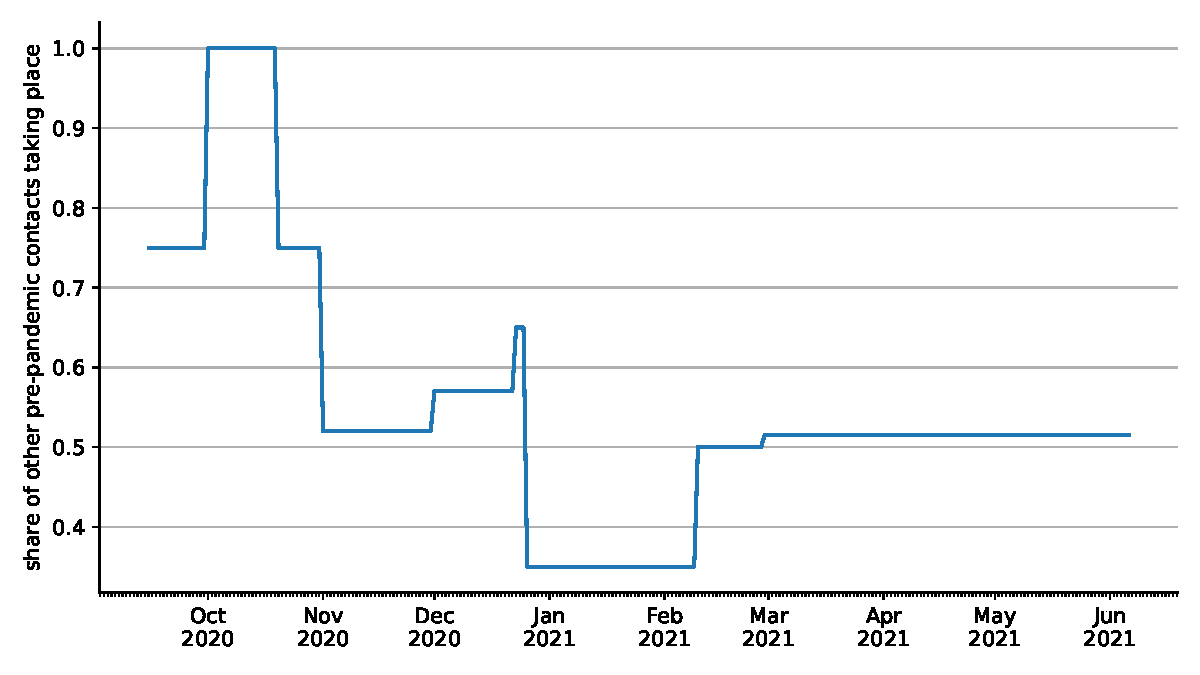
\includegraphics[width=\textwidth]{figures/results/figures/data/other_multiplier}
    \caption{Share of Pre-Pandemic Other Contacts Taking Place with Infection Potential}
    \label{fig:other_multiplier}
    \floatfoot{\noindent \textit{Note:} All values are estimated. We try to use as little
    switching points as possible and tie them to political events (such as lockdown
    announcements) unless changes are used to capture anticipation or pandemic fatigue
    (for example we model an anticipation of the November lockdown and model lockdown
    fatigue in early March).}
\end{figure}

% seasonality
Another potentially important factor for a contact to lead to an infection is the
seasonality \citep{Kuehn2020, Carlson2020} There are two channels through which
seasonality affects the infectiousness of contacts. One has to do with the physical
conditions like the temperature and the humidity. The other has to do with where people
meet. Especially leisure contacts are more likely to take place outdoors and individuals
are more likely to have windows open when the weather is nicer. To capture both channels
we allow for other contacts to have a higher seasonality than our other contact models.
Figure~\ref{fig:seasonality} shows our seasonality factors.

\begin{figure}
    \centering
    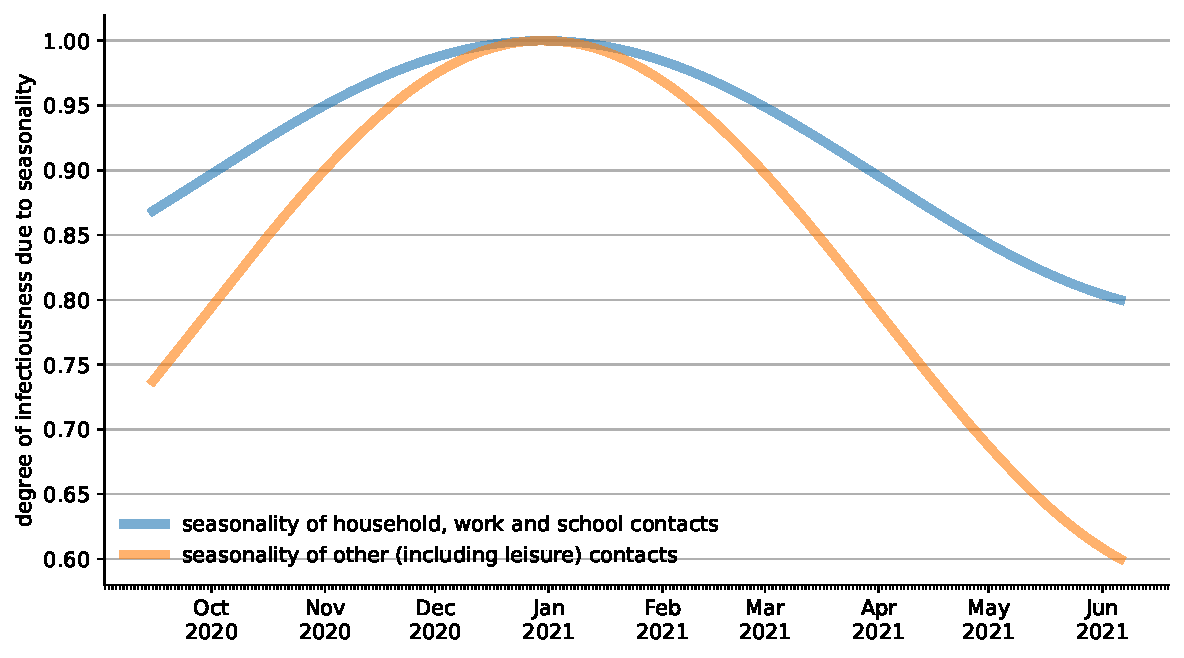
\includegraphics[width=\textwidth]{figures/results/figures/data/seasonality}
    \caption{Seasonality by Type of Contact}
    \label{fig:seasonality}
    \floatfoot{\noindent \textit{Note:} We model seasonality as a factor that reduces the
    probability of infection of all encounters. The factor depends on the day and is
    calculated from a sinus shaped function with its maximum on January 1st. Since
    seasonality can affect the transmission both through physical conditions such as
    temperature and humidity as well as through the numbers of contacts that take place
    outside we assume two seasonality factors. One for other contacts which we expect to
    be strongly affected by fairer weather with a maximum reduction of 42\% in the
    infection probability. The other seasonality only makes contacts up to 21\% less
    infectious and is applied to household, work and school contacts.}
\end{figure}



\FloatBarrier


In our model, there are five reasons why rapid tests are done:\comment[id=J]{Add a
section on how we calibrate rapid test demand; Mainly describe the datapoints we have and
say that we usually interpolate linearly in between data points. (Only exception to that
is private rapid test demand, which we fit to data)}

\begin{enumerate}
    \item someone plans to have work contacts
    \item someone is an employee of an educational facility or a school pupil
    \item a household member has tested positive or developed symptoms
    \item someone has developed symptoms but has not received a PCR test
    \item someone plans to participate in a weekly non-work meeting
\end{enumerate}

\subsubsection{work rapid tests}

For work contacts, we know from the COSMO study (\cite{Betsch2021}, 20th/21st of April)
that 60\% of workers who receive a test offer by their employer regularly use it. We
assume this share to be time constant.

In addition, there are some surveys that allow us to trace the expansion of employers who
offer tests to their employees. Mid march, 20\% of employers offered tests to their
employees \citep{DIHK2021}. In the second half of March, 23\% of employees reported being
offered weekly rapid tests by their employer \citep{Ahlers2021}. This share increased to
60\% until the first days of April \cite{ZDF2021}.

\textcolor{red}{ToDo: Find the survey that the ZDF is citing here}

Until mid April 70\% of workers were expected to receive a
weekly test offer \citep{AerzteZeitung2021}. However, according to surveys conducted in
mid April \citep{Betsch2021}, less than two thirds of individuals with work contacts
receive a test offer. Starting on April 19th employers were required by law to provide
two weekly tests to their employees \citep{Bundesanzeiger2021}. We assume that compliance
is incomplete and only 80\% of employers actually offer tests.

\subsubsection{educ rapid tests}

We assume that employees in educational facilities start getting tested in 2021 and that
by March 1st 30\% of them are tested weekly. The share increases to 90\% for the week
before Easter. At that time both Bavaria \citep{BayrischerRundfunk2021} and
Baden-Württemberg \citep{MinisteriumKultus2021} were offering tests to teachers and
North-Rhine
Westphalia\footnote{\url{https://www.land.nrw/de/pressemitteilung/umfassende-informationen-fuer-die-schulen-zu-corona-selbsttests-fuer-schuelerinnen}}
\cite{DPA2021} and Lower Saxony \citep{SueddeutscheZeitung2021} were already testing
students and tests for students and teachers were already mandatory in Saxony
\citep{SueddeutscheZeitung2021a}. After Easter we assume that 95\% of teachers get tested
twice per week.

Tests for students started
later\footnote{\url{https://www.land.nrw/de/pressemitteilung/umfassende-informationen-fuer-die-schulen-zu-corona-selbsttests-fuer-schuelerinnen}}
\citep{MinisteriumKultus2021} so we assume that they only start in February and only 10\%
of students get tested by March 1st. Relying on the same sources as above we approximate
that by the week before Easter this share had increased to 40\%.\footnote{\url{https://www.land.nrw/de/pressemitteilung/umfassende-informationen-fuer-die-schulen-zu-corona-selbsttests-fuer-schuelerinnen}, }

After Easter the share of students receiving twice weekly tests is set to 75\%. This as
based on tests becoming mandatory becoming mandatory in Bavaria after Easter
break\footnote{Bavaria\footnote{\url{https://bit.ly/3nz5fXS}}, in North-Rhine Westphalia
on April
12th\footnote{https://www.schulministerium.nrw/ministerium/schulverwaltung/schulmail-archiv/14042021-schulbetrieb-im-wechselunterricht-ab-montag},
\url{https://bit.ly/2QHilX3}} and on the 19th in
Baden-Württemberg\footnote{https://bit.ly/3vuetaD, https://bit.ly/3vuetaD}.


To limit our degrees of freedom, we only have one parameter that governs how many
individuals do a rapid test because of any of the private demand reasons (own symptoms
but no PCR test, planned weekly leisure meeting or a symptomatic or positively tested
household member).

We assume that there is no private rapid test demand until March when both the citizens'
tests and rapid tests for lay people started to become available
\footnote{\url{https://bit.ly/3ehmGcj}, \url{https://bit.ly/3xJCIn8}} and other access to
rapid tests was very limited.

According to the COSMO study\footnote{\url{https://bit.ly/2QSFAgR}} 63\% would have been
willing to take a test in the round of 23rd of February 2021 when an acquaintance would
have tested positive. Since this is only asking for willingness not actual behavior and
the demand when meeting with friends is very likely lower, we take this as the upper
bound of private rapid test demand which is reached on May 4th. To cover that many people
are likely to have sought and done their first rapid test before the Easter holidays to
meet friends or family, we let the share of individuals doing rapid tests in that time
increase more rapidly than before and after. By end of March 25\% of individuals would do
a rapid test due to a private reason.



All shares of individuals who would take a rapid test if the conditions were met can be
seen in Figure~\ref{fig:rapid_test_demand}.

\begin{figure}
    \centering
    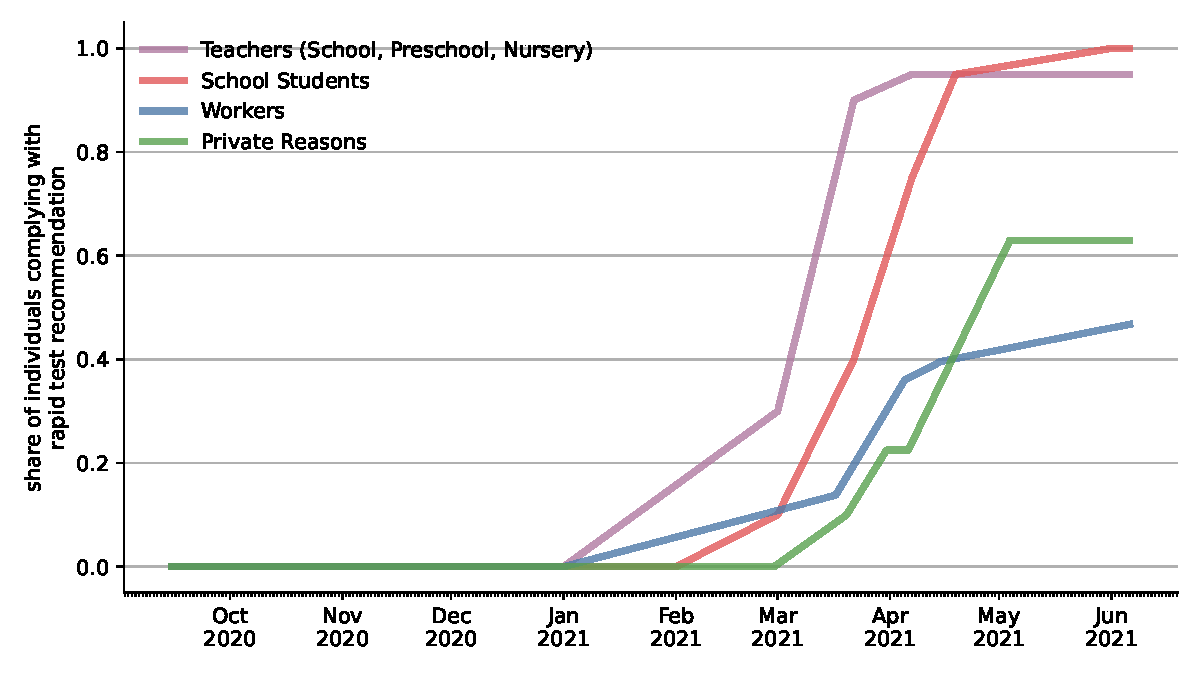
\includegraphics[width=\textwidth]{figures/results/figures/data/testing/rapid_test_demand_shares}
    \caption{\textbf{Share of Individuals Doing a Rapid Test.}}
    \floatfoot{\noindent \textit{Note:} Rapid test demand can be triggered by individuals
    planning to have education contacts, work contacts, developing symptoms without
    access to a PCR test, having a household member with a positive test or symptoms. In
    each case whether a rapid test is done depends on how long it has been since the
    individual's last rapid test and her individual compliance parameters. As an example,
    take a worker in May. In that time workers are encouraged to test themselves twice
    weekly but there is no general requirement to test themselves. If the worker has not
    done a test within the last four days in our model she will demand a test if her
    (time-constant) compliance parameter belongs to the upper 60\% in the population.}
    \label{fig:rapid_test_demand}
\end{figure}


\begin{figure}[ht]
    \centering
    \caption{Share of Individuals With Rapid Tests}
    \label{fig:share_ever_rapid_test}
    \begin{subfigure}{.55\textwidth}
        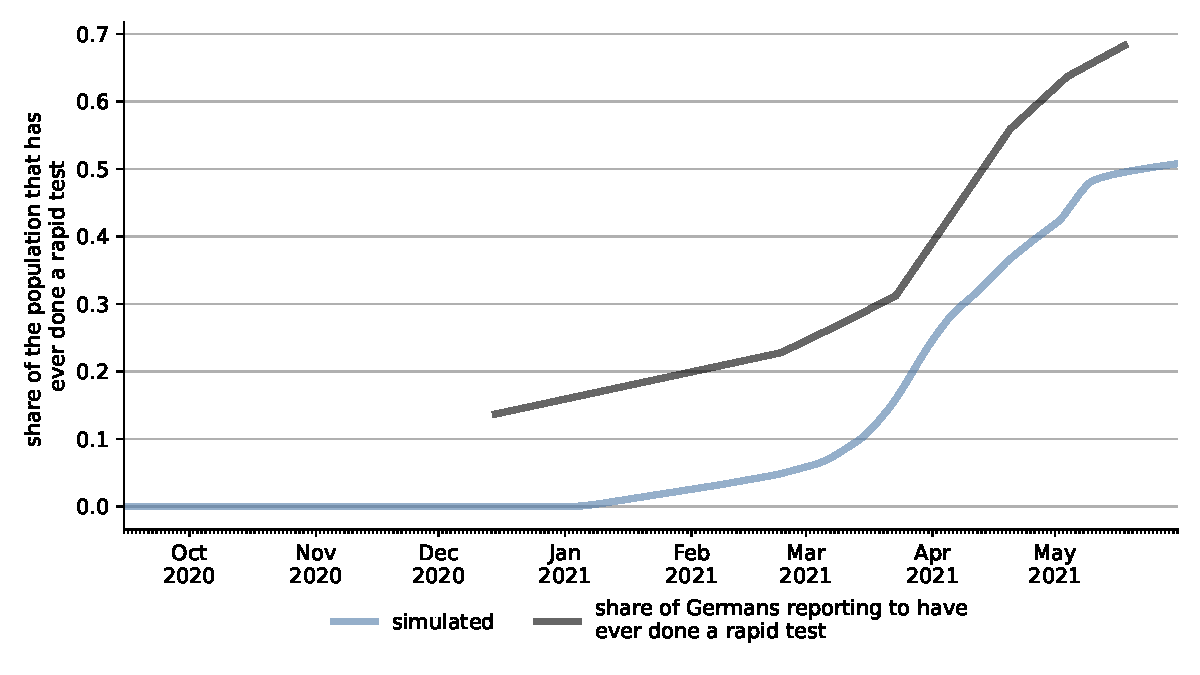
\includegraphics[width=0.9 \textwidth]{figures/results/figures/scenario_comparisons/combined_fit/full_share_ever_rapid_test}
        \caption{Share of Individuals That Have Ever Done a Rapid Test}
    \end{subfigure}%
    \begin{subfigure}{.55\textwidth}
        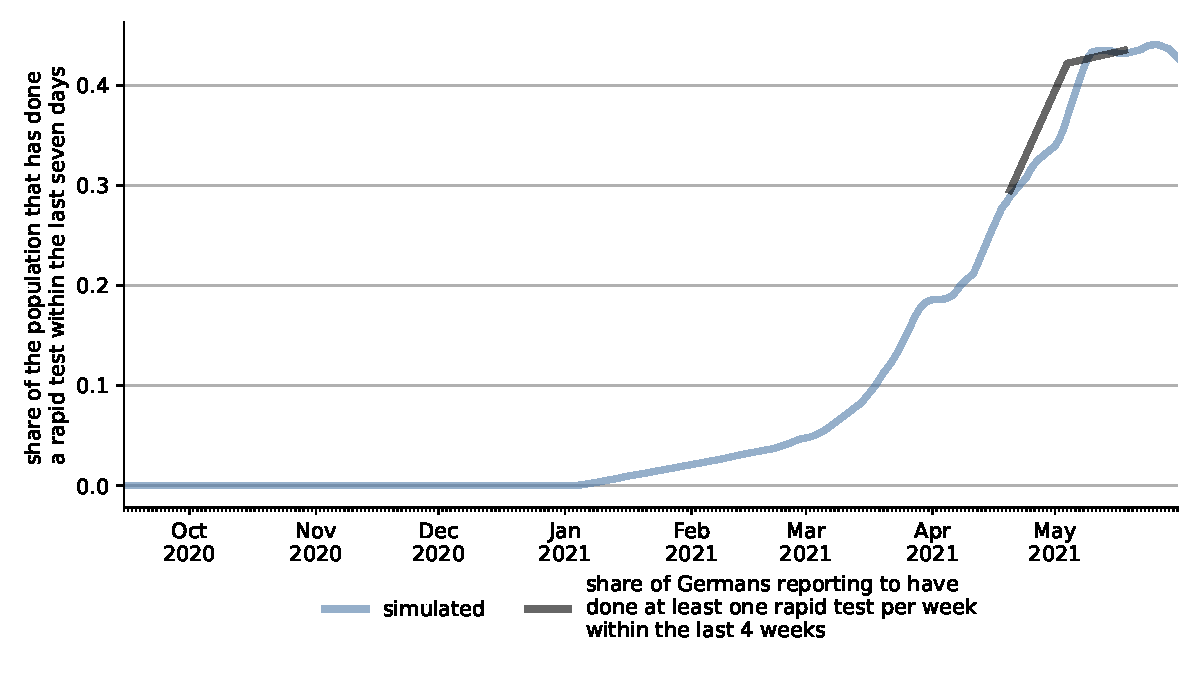
\includegraphics[width=0.9 \textwidth]{figures/results/figures/scenario_comparisons/combined_fit/full_share_rapid_test_in_last_week}
        \caption{Share of Individuals Having Done a Rapid Test in the Last Week}
    \end{subfigure}
    \label{fig:share_rapid_test_last_week}
    \floatfoot{\noindent \textit{Note:} The figure compares the share of individuals who
        have ever done a rapid test or done a rapid test within the last week in our
        simulations to the shares reported in the
        \href{https://projekte.uni-erfurt.de/cosmo2020/web/topic/wissen-verhalten/80-schnelltests/}{COVID-19
        Snapshot Monitoring Survey}. The left panel compares the share of individuals who
        have ever done a rapid test. The right panel compares the share of individuals
        who have done a rapid test within the last seven days in our simulation compared
        to the share reporting to have done at least weekly rapid tests in the last four
        weeks in the COSMO survey. Overall our calibration of rapid tests are slightly
        conservative. The overall share is below that in the study. We fit the share of
        weekly tests quite exactly. However, the study only covers adults while our share
        also includes children who are tested very regularly when attending school.}
\end{figure}

 \comment[id=K]{J: Explain that we don't fit the share ever tested that well because our rapid test compliance is completely fixed. }